\subsection{Arquitectura física}
Después de haber realizado el análisis del funcionamiento del sistema a partir de la división de la función principal en varias subfunciones y de conocer la interrelación que existe en cada una de ellas, es posible agruparlas en diferentes módulos y sistemas. 

Para lograr dicho cometido, se utilizará el SPA (System Physical Architecture), que es la representación de la transformación de funciones en sistemas, subsistemas, ensambles y componentes físicos. \cite{Flores2018} Estos sistemas deben estar ligados a las funciones del dominio funcional y cumplir con los requerimientos del sistema para asegurar el correcto funcionamiento del prototipo.

Para plantear el modelo, se parte de una arquitectura genérica para sistemas mecatrónicos, que servirá como referencia para la construcción de la arquitectura física del sistema. (Figura \ref{fg:ArchFis})

\textbf{Sistema de administración de comportamiento $(S_1)$}: Este sistema se encargará de la toma de decisiones del sistema, a través de un módulo de análisis de información $(M_{11})$, el cual se encarga de analizar los datos obtenidos del sistema $(S_2)$; a su vez tomará las decisiones $(M_{12})$ para regular las acciones de cada sistema. 

\textbf{Sistema de procesamiento de datos $(S_2)$}: Este sistema se encargará de adquirir los datos internos y externos que son necesarios para controlar el sistema. Cuenta con un módulo para adquirir datos$(M_{21})$ que se obtienen a través de sensores colocados en el sistema $(S_5)$ y también de la interfaz Humano-Máquina del sistema $S_6$, al mismo tiempo estos datos pasan por la etapa de Acondicionamiento de señales $(M_{22})$, el cual prepara los datos para poder ser trabajados en el sistema $S_1$. Este último contará con un módulo de Comunicación $(M_{23})$ el cual se encargará de transmitir las señales procesadas a todos los sistemas que lo requieran. También se cuenta con un Módulo de Interfaz Humano-Máquina $(M_{24})$, que sirve para la interacción del usuario con el sistema mecatrónico.

\textbf{Sistema de energía $(S_3)$}: Este sistema se encargará de la administración de la energía eléctrica dentro del dispositivo. Primero pasa por un Módulo de transformación $(M_{31})$, que es el encargado de transformar la energía, ya sea regulación de AC o transformándola en DC, según se requiera en el dispositivo. Pasa al módulo encargado de Regular la tensión $(M_{32})$ para los dispositivos electrónicos de los sistemas $S_1$ y $S_2$, así como transmitir la energía necesaria para la alimentación de los motores $(M_{33})$ para los sistemas $S_4$ y $S_5$.

\textbf{Sistema de trituración de residuos $(S_4)$}: Este sistema se encargará de reducir el tamaño de los residuos suministrados.

\textbf{Sistema de procesamiento $(S_5)$}: Este es el sistema donde se llevará a cabo la mayor parte del proceso de compostaje, empezando por el módulo de aireación $(M_{51})$ el cual se encargará de mezclar los residuos y de permitir la oxigenación de la mezcla; a su vez, contará con el módulo de autorregulación $(M_{52})$ el cual recibe los datos gestionados del $S_1$ y realiza los procesos para regular el ambiente del proceso.

%\textbf{Sistema de Comunicación Externa}: Este sistema cuenta el modulo de Recepción de instrucciones $(M_{61})$ el cual se encarga de recibir las instrucciones del usuario y también cuenta con un modulo de Comunicación de datos $(M_{62})$ el cual muestra los datos sobre el proceso y las variables del ambiente al usuario. 

La interconexión de los diferentes módulos del dispositivo se puede observar en la figura \ref{fg:ArchFis}

\begin{figure}[h!]
            \centering
            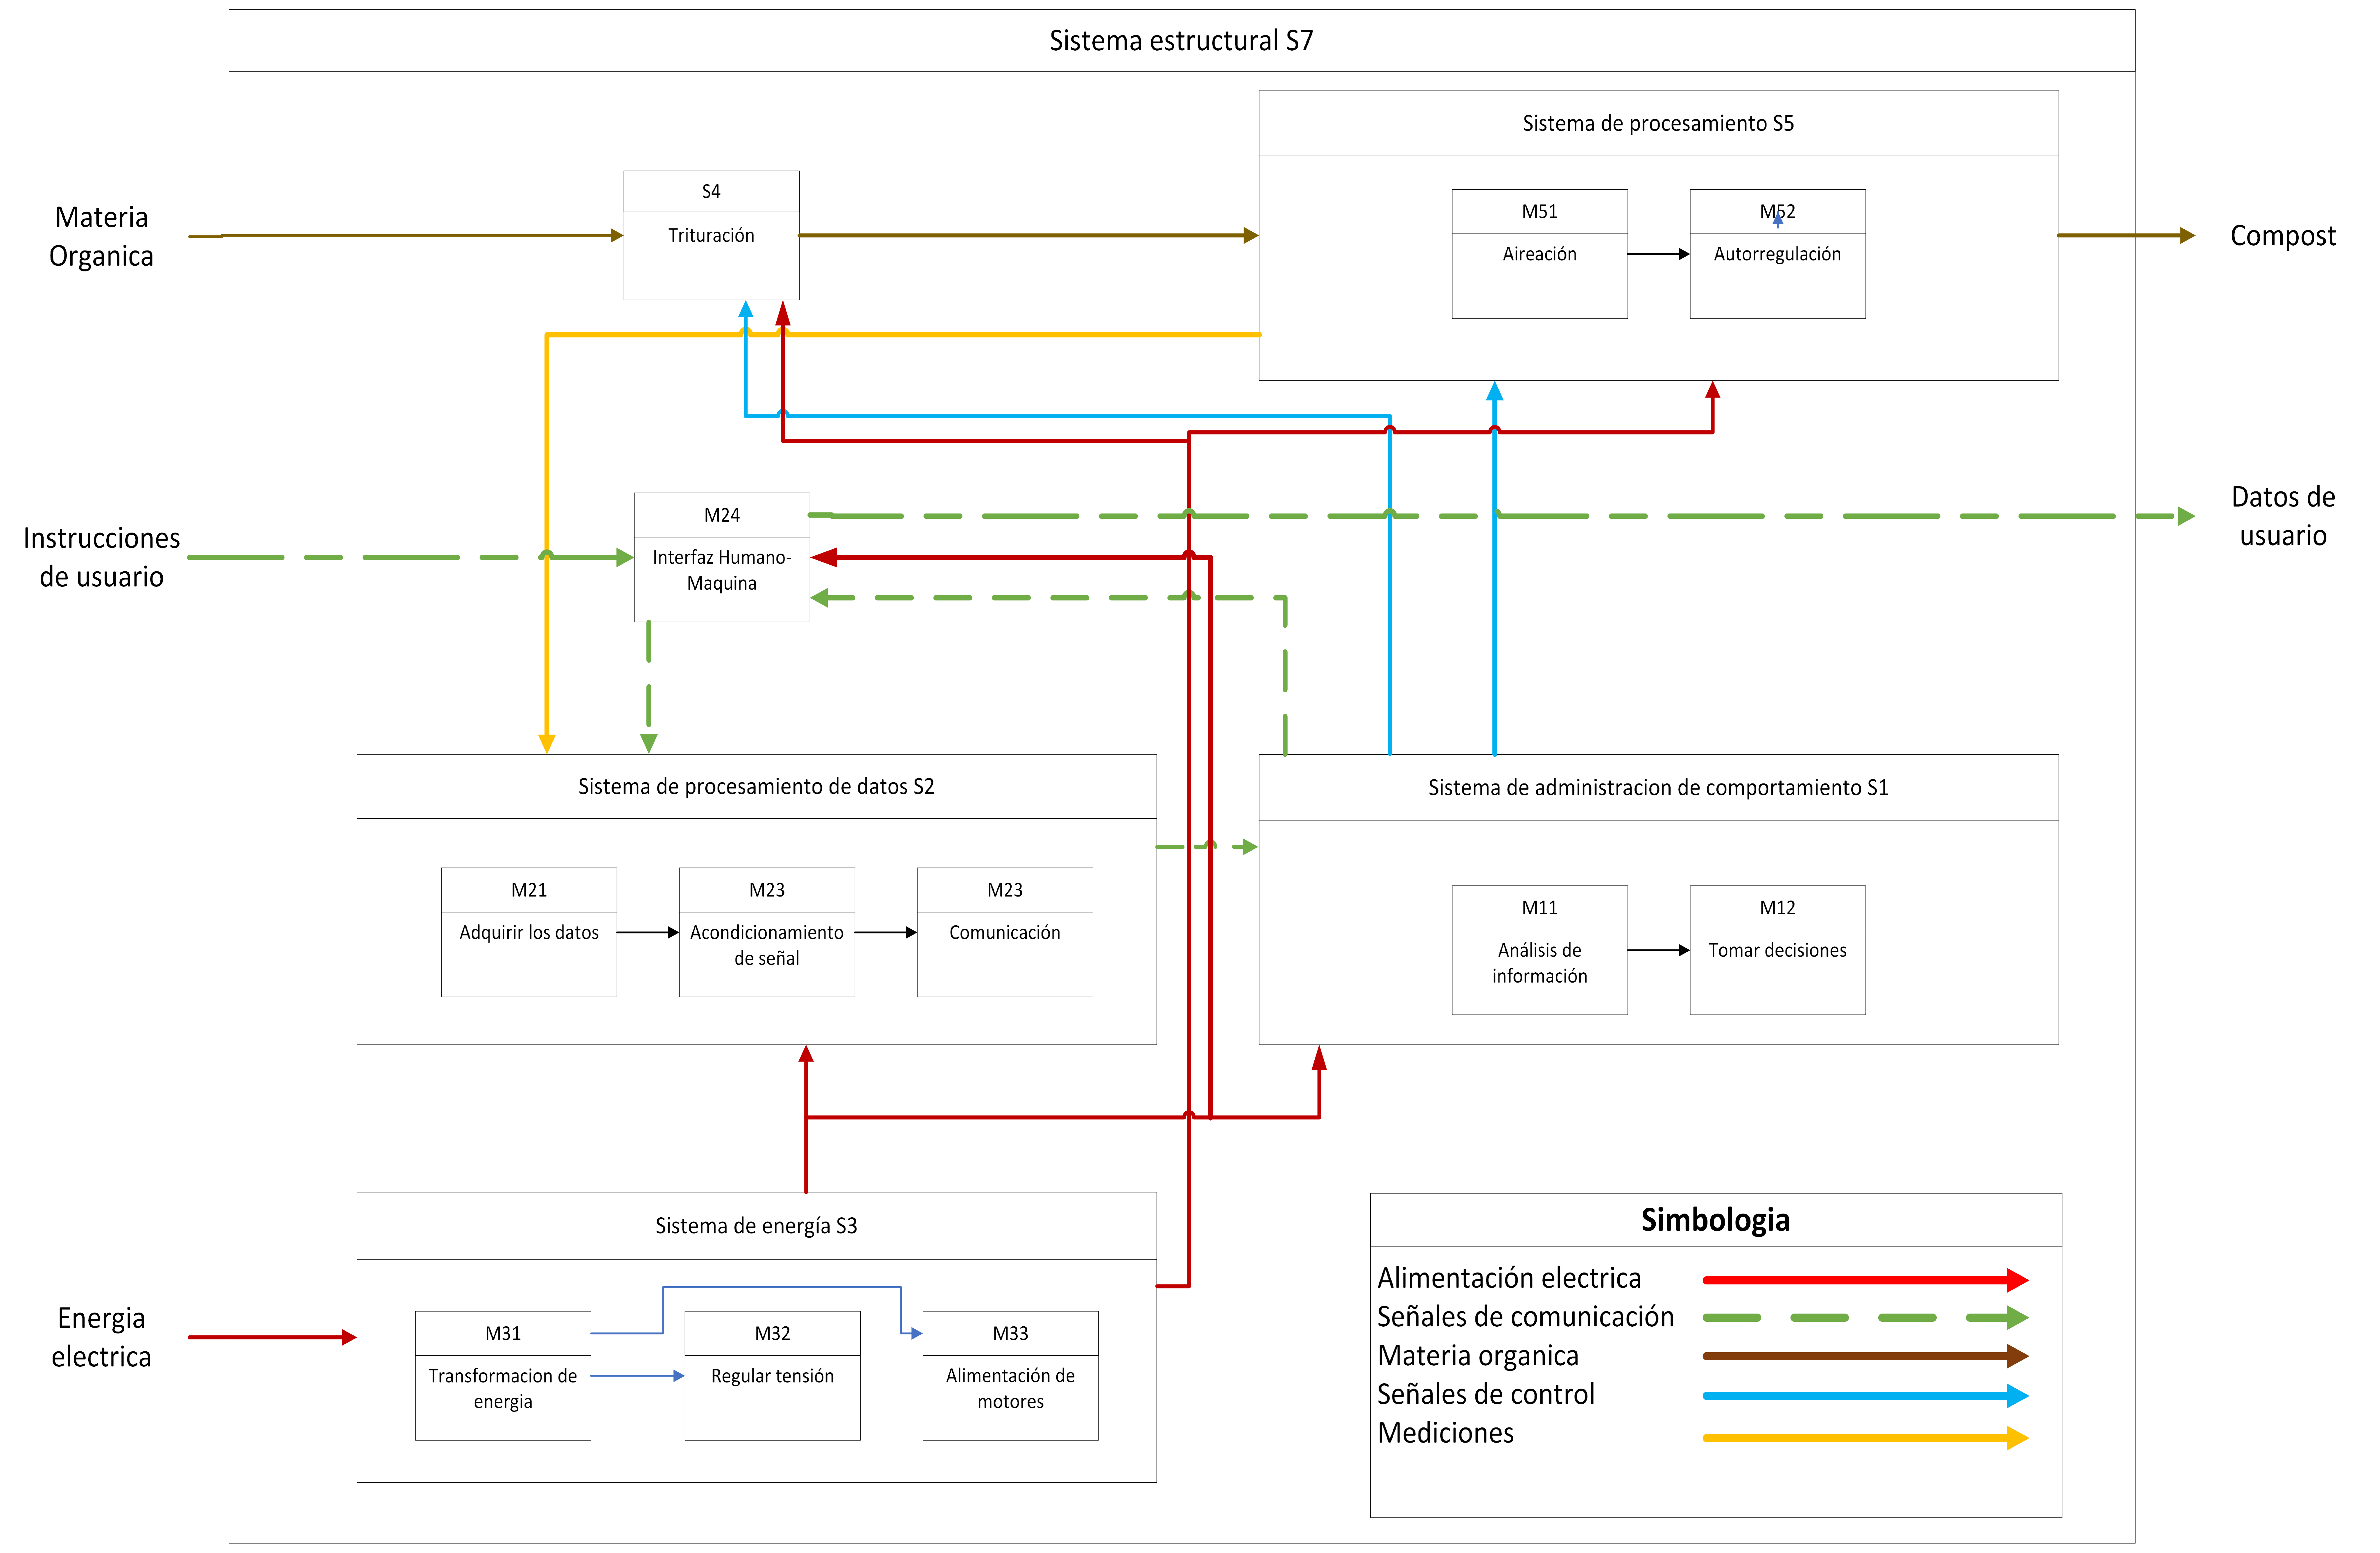
\includegraphics[scale=0.2, angle = 90]{images/Capitulo 3/3.1.1.3 Arquitectura fisica/Arquitectura fisica.png}
            \caption{Arquitectura física propuesta}
            \label{fg:ArchFis}
        \end{figure}

\newpage